\documentclass[trans]{beamer}
\usepackage{etex}
\usepackage{amsthm}
\usepackage{xcolor}
\usepackage{wrapfig}
\usepackage{soul}
\usepackage{lipsum}
\usepackage{booktabs}
\usepackage{graphicx}
\usepackage{algorithm}
\usepackage{algorithmic}
\usepackage{answers}
\usepackage[absolute,overlay]{textpos}
\usepackage{verbatim}
\usepackage{fancyvrb}
\usepackage{xspace}
%\usepackage[labelsep=none]{caption}
\usepackage{tikz}
\usepackage{units}
\usepackage{makeidx}
\usepackage{tabularx}
\usepackage{colortbl}
\usepackage{multirow}
\usepackage{calc}
%\usepackage{graphicx}
%\usepackage{array}
%\usepackage[all]{xy}
%%\usepackage{theapa}
%\usepackage{tikz}
%\usetikzlibrary{shapes.geometric} 
%\usetikzlibrary{shadows} 
%\usetikzlibrary{positioning}
%\usepackage{algorithm}
%%\usepackage{algorithmic}
%\usepackage{algorithmic}
%%\usepackage{algpseudocode}
%\usepackage{natbib}
%\usepackage{apalike}
\usepackage{../book/haldefs}

\mode<presentation>
{
%  \usetheme{AnnArbor}
%  \usetheme{Antibes}
%  \usetheme{Bergen}
%  \usetheme{Berkeley}
%  \usetheme{Berlin}
%  \usetheme{Boadilla}
%  \usetheme{boxes}
%  \usetheme{CambridgeUS}
%  \usetheme{Copenhagen}
%  \usetheme{Darmstadt}
%  \usetheme{default}
%  \usetheme{Dresden}
%  \usetheme{Frankfurt}
%  \usetheme{Goettingen}
%  \usetheme{Hannover}
%  \usetheme{Ilmenau}
%  \usetheme{JuanLesPins}
%  \usetheme{Luebeck}
%  \usetheme{Madrid}
%  \usetheme{Malmoe}
%  \usetheme{Marburg}
%  \usetheme{Montpellier}
%  \usetheme{PaloAlto}
%  \usetheme{Pittsburgh}
%  \usetheme{Rochester}
%  \usetheme{Singapore}
%  \usetheme{Szeged}
%  \usetheme{Warsaw}
  \usetheme{Unife}

%\usecolortheme{lily}% 
  % or ...

  \setbeamercovered{transparent}
  % or whatever (possibly just delete it)
}


\usepackage[english]{babel}
% or whatever

%\usepackage[latin1]{inputenc}
% or whatever
\usetikzlibrary{shapes,snakes}
%%% Local Variables: 
%%% mode: latex
%%% TeX-master: "courseml"
%%% End: 

%%%%%%%%%%% COLORS

\definecolor{darkgrey}{rgb}{0.2,0.2,0.2}
\definecolor{grey}{rgb}{0.9,0.9,0.9}
\definecolor{darkblue}{rgb}{0.0,0.0,0.5}
\definecolor{darkpurple}{rgb}{0.4,0.0,0.4}
\definecolor{darkred}{rgb}{0.5,0.0,0.0}
\definecolor{darkorange}{rgb}{0.5,0.45,0.4}
\definecolor{darkgreen}{rgb}{0.0,0.5,0.0}
\definecolor{darkergreen}{rgb}{0.0,0.4,0.0}
\definecolor{lightblue}{rgb}{0.8,0.8,1.0}
\definecolor{lightgreen}{rgb}{0.8,1.0,0.8}
\definecolor{lightred}{rgb}{1.0,0.8,0.8}
\definecolor{lightyellow}{rgb}{1.0,1.0,0.8}
\definecolor{lightorange}{rgb}{1.0,0.9,0.8}
\definecolor{lightgrey}{rgb}{0.96,0.97,0.98}
\definecolor{Sepia}{HTML}{671800}

%%%%%%%%%%%%% FORMATTING
%
%\newcommand*\chapterlabel{}
%\makeatletter
%\titleformat{\chapter}%
%  [block]                                % shape
%  {\gdef\chapterlabel{}
%   \normalfont\sffamily\Huge\bfseries\scshape}            % format applied to label+text
%  {\gdef\chapterlabel{\thechapter~|~}}    % 
%  {0pt}                                  % horizontal separation between label and title body
%  {\begin{tikzpicture}[remember picture,overlay]
%    \node[yshift=-3cm] at (current page.north west)
%      {\begin{tikzpicture}[remember picture, overlay]
%        \draw[fill=lightgreen] (0,0) rectangle
%          (\paperwidth,3cm);
%        \node[anchor=east,xshift=.9\paperwidth,rectangle,
%              rounded corners=20pt,inner sep=11pt,
%              fill=darkergreen]
%              {\color{white}\chapterlabel#1};
%       \end{tikzpicture}
%      };
%   \end{tikzpicture}
%  }% before the title body
%  []%after the title body
%\makeatother 
%%\titlespacing*{\chapter}{0pt}{50pt}{-10pt}
%
%\newcommand{\sectionsize}{}
%\titleformat{\section}%
%  [hang]% shape
%  {\normalfont\Large\itshape}% format applied to label+text
%  {\textcolor{darkergreen}{\makebox[0pt][r]{\thesection\quad }#1}}% label
%  {1em}% horizontal separation between label and title body
%  {}% before the title body
%  []% after the title body
%
%\titleformat{\subsection}%
%  [hang]% shape
%  {\normalfont\large\itshape}% format applied to label+text
%  {\textcolor{darkergreen}{\makebox[0pt][r]{\thesubsection\quad }#1}}% label
%  {1em}% horizontal separation between label and title body
%  {}% before the title body
%  []% after the title body



%%%%%%%%%%% EXERCISE STUFF

\newtheorem{Ex}{Exercise}
\newenvironment{exercises}{\section{Exercises}}{}
% \center\begin{tabular}{c}\hline{\bf\Large Exercises}\\\hline\end{tabular}}{}

%\Newassociation{solution}{Soln}{solutions}
%\Newassociation{hint}{Hint}{solutions}
\newcommand{\prehint}{~[Hint]}
\newcommand{\presolution}{}
\newcommand{\Opensolutionshook}[2]%
  {\Writetofile{#1}{}}
%\renewcommand{\Solnlabel}[1]{%
%  {\Large\linespread{1}%
%  \begin{tabular}{|p{\textwidth}@{}|}%
%    \hline%
%    \emph{Solution #1}\\%
%    \hline%
%  \end{tabular}\newline}}
%\renewcommand{\Hintlabel}[1]{\emph{Hint #1}}


\newcommand{\emptylist}{[ ]}
\newcommand{\pushlist}[1]{{\ensuremath \oplus} #1}

\newcommand*\learningproblemargument{}
\newsavebox{\learningproblembox}
\newenvironment{learningproblemenv}[1]
  {\gdef\learningproblemargument{#1}\begin{lrbox}{\learningproblembox}\begin{minipage}{4in}}
  {\end{minipage}\end{lrbox}%
   \tikzstyle{mybox} = [draw=darkgreen, fill=green!5, very thick, rectangle, rounded corners, inner sep=10pt, inner ysep=12pt]%
   \tikzstyle{fancytitle} =[fill=darkgreen, text=white, rectangle, rounded corners]%
   \vspace{1em}
   \noindent
   \begin{tikzpicture}
     \node [mybox] (box) {\usebox{\learningproblembox}};
     \node [fancytitle, right=10pt] at (box.north west) {\normalfont\sffamily\Large\bfseries\scshape Task: \learningproblemargument};
   \end{tikzpicture}
  }

\newcommand{\learningproblem}[3]{
  \begin{learningproblemenv}{#1}
    \emph{Given:}
    \begin{enumerate}
      #2
    \end{enumerate}
    \emph{Compute:} #3
  \end{learningproblemenv}}

\newcommand{\lprob}[1]{{\normalfont\sffamily\scshape #1}}

%%%%%%%%%%% ENVIRONMENTS

\DefineVerbatimEnvironment%
  {chapternotes}{Verbatim}
  {baselinestretch=1.0,frame=single,fillcolor=\color{lightgreen}}
%\renewenvironment{chapternotes}{\begin{comment}}{\end{comment}}

\newenvironment{editedout}{\begin{comment}}{\end{comment}}

\newenvironment{derivation}
  {\begin{eqnarray}}
  {\end{eqnarray}}

\newcommand{\derivstep}[2]{#1\sidenote{#2}}

%\makeatletter\newenvironment{learninggoals}{%
%   ~\\\noindent\begin{lrbox}{\@tempboxa}\begin{shadowblock}{\columnwidth}\begin{itemize}}{\end{itemize}\end{shadowblock}\end{lrbox}%
%   {\usebox{\@tempboxa}}
%}\makeatother

%\newenvironment{learningobjectives}
%  {\begin{marginfigure}\begin{learninggoals}\item[]\item[] \hspace{-2em} {\bf Learning Objectives:}}
%  {\end{learninggoals}\end{marginfigure}}

\newsavebox{\objectivesbox}
\newlength{\objectivesheight}
\newenvironment{learningobjectives}
  {\begin{lrbox}{\objectivesbox}\begin{minipage}{2in}\vspace{2pt}{\bf Learning Objectives:}\begin{footnotesize}\begin{itemize}}
  {\end{itemize}\end{footnotesize}\end{minipage}\end{lrbox}\begin{textblock}{2}(10.2,2.5)\begin{shadowblock}{2in}\usebox{\objectivesbox}\end{shadowblock}\end{textblock}\settoheight{\objectivesheight}{\usebox{\objectivesbox}}}

\newenvironment{chapterintro}
  {}
  {}

\newcommand*\vignetteargument{}
\newsavebox{\vignettebox}
\newenvironment{vignette}[1]
  {\gdef\vignetteargument{#1}\begin{lrbox}{\vignettebox}\begin{minipage}{6.4in}}
  {\end{minipage}\end{lrbox}%
   \tikzstyle{mybox} = [draw=Periwinkle, fill=Periwinkle!5, very thick, rectangle, rounded corners, inner sep=10pt, inner ysep=12pt]%
   \tikzstyle{fancytitle} =[fill=Periwinkle, text=white, rectangle, rounded corners]%
   \vspace{1em}
   \noindent
   \begin{tikzpicture}
     \node [mybox] (box) {\usebox{\vignettebox}};
     \node [fancytitle, right=10pt] at (box.north west) {\normalfont\sffamily\Large\bfseries\scshape Vignette: \vignetteargument};
   \end{tikzpicture}
  }

%[transform shape, baseline=-3.5cm]
\newcommand*\mathreviewargument{}
\newsavebox{\mathreviewbox}
\newenvironment{mathreview}[1]
  {\gdef\mathreviewargument{#1}\begin{lrbox}{\mathreviewbox}\begin{minipage}{6.4in}}
  {\end{minipage}\end{lrbox}%
   \tikzstyle{mybox} = [draw=Sepia, fill=Sepia!5, very thick, rectangle, rounded corners, inner sep=10pt, inner ysep=12pt]%
   \tikzstyle{fancytitle} =[fill=Sepia, text=white, rectangle, rounded corners]%
   \begin{figure*}[t]
     \begin{tikzpicture}
       \node [mybox] (box) {\usebox{\mathreviewbox}};
       \node [fancytitle, right=10pt] at (box.north west) {\normalfont\sffamily\Large\bfseries\scshape Math Review | \mathreviewargument};
     \end{tikzpicture}
     \caption[Math Review: \mathreviewargument]{~}
   \end{figure*}%
  }


%\newenvironment{chapterquote}
%  {\textblockcolor{grey}\begin{textblock}{6.5}(8,1)}
%  {\end{textblock}}

%\newenvironment{chapterimage}
%  {\textblockcolor{white}\begin{textblock}{6.5}(8,1)}
%  {\end{textblock}}


%  {\par\linespread{1}\center%
%   \begin{greybox}%
%   \begin{tabular}{|p{4in}|}%
%     \hline\vspace{+0.02in}%
%     \rule{1ex}{1ex} Learning Goals \rule{1ex}{1ex}%
%     }
%  { \vspace{+0.05in}\\\hline%
%   \end{tabular}\vspace{+0.1in}\end{greybox}\\}\makeatother


%%%%%%%%%%% COMMANDS

\newcommand{\bigemph}[1]{\textcolor{darkblue}{\bf #1}}

\newcommand{\dependencies}[1]{\marginnote[2.5in]{Dependencies: #1}}

%\newcommand{\dependencies}[1]{\begin{textblock}{2}(10.2,2.5)Dependencies: #1\end{textblock}}

%\sethlcolor{lightyellow}

\newcommand{\concept}[1]{\hl{\bf #1}\index{#1}}
\newcommand{\koncept}[2]{\hl{\bf #1}\index{#2}}

\newcommand{\chref}[1]{Chapter~\ref{#1}}


\newcommand{\chapterquote}[2]
  {\tikzstyle{mybox} = [draw=darkergreen, fill=green!20, very thick, rectangle, rounded corners, inner sep=5pt, inner ysep=5pt]
   \tikzstyle{fancytitle} =[fill=darkergreen, text=white]
   \begin{textblock}{7.5}(2,2.5)
   \begin{tikzpicture}[transform shape, rotate=0, baseline=-3.5cm]
   \noindent%
   \node [mybox] (box) {%
    \begin{minipage}[t!]{\textwidth}
      \noindent%
      \begin{large}%
      \textsf{#1}%
      \end{large}
      \hfill\textcolor{darkergreen}{\textsf{--~#2}}
    \end{minipage}
    };
%   \node[fancytitle] at (box.south) {\emph{-- #2}};
  \end{tikzpicture}
  \end{textblock}}

\newcommand{\chapterimage}[2]
  {\tikzstyle{mybox} = [draw=darkergreen, fill=green!20, very thick, rectangle, rounded corners, inner sep=5pt, inner ysep=5pt]
   \tikzstyle{fancytitle} =[fill=darkergreen, text=white]
   \begin{textblock}{7.5}(2,2.5)
   \begin{tikzpicture}[transform shape, rotate=0, baseline=-3.5cm]
   \noindent
   \node [mybox] (box) {%
    \begin{minipage}[t!]{\textwidth}
      \includegraphics[width=\textwidth]{#1}

      \hfill\textcolor{darkergreen}{\textsf{--~#2}}
    \end{minipage}
    };
%   \node[fancytitle] at (box.south) {\emph{-- #2}};
  \end{tikzpicture}
  \end{textblock}}

\newcommand{\chapterimageopt}[3]
  {\tikzstyle{mybox} = [draw=darkergreen, fill=green!20, very thick, rectangle, rounded corners, inner sep=5pt, inner ysep=5pt]
   \tikzstyle{fancytitle} =[fill=darkergreen, text=white]
   \begin{textblock}{7.5}(2,2.5)
   \begin{tikzpicture}[transform shape, rotate=0, baseline=-3.5cm]
   \noindent
   \node [mybox] (box) {%
    \begin{minipage}[t!]{\textwidth}
      \includegraphics[#2]{#1}

      \hfill\textcolor{darkergreen}{\textsf{--~#3}}
    \end{minipage}
    };
%   \node[fancytitle] at (box.south) {\emph{-- #2}};
  \end{tikzpicture}
  \end{textblock}}


\newcommand{\monthyear}{%
  \ifcase\month\or January\or February\or March\or April\or May\or June\or
  July\or August\or September\or October\or November\or
  December\fi\space\number\year
}

\newcommand{\blankpage}{\newpage\hbox{}\thispagestyle{empty}\newpage}
\newcommand{\mycite}[1]{\ e{\citealt{#1}}}
\newcommand{\bookurl}{\url{http://hal3.name/courseml/}}

\newcommand{\TODOFigure}[2]{%
  \begin{marginfigure}
    \framebox[\textwidth][c]{\begin{minipage}{\textwidth}\rule{0pt}{2in}\end{minipage}}
    \caption{{\tt #1}: #2}
    \label{fig:#1}
  \end{marginfigure}}

\newlength{\NextFigureOffset}
\newcommand{\ResetNextFigure}{\setlength{\NextFigureOffset}{0mm}}
\newcommand{\MoveNextFigure}[1]{\setlength{\NextFigureOffset}{#1}}

\ResetNextFigure{}

\newcommand{\Figure}[2]{%
  \begin{marginfigure}[\NextFigureOffset]
    \begin{centering}
    \includegraphics[width=\textwidth]{figs/#1}
    \caption{#2}
    \label{fig:#1}
    \end{centering}
  \end{marginfigure}
  \ResetNextFigure{}
  }

\newcommand{\Table}[4]{%
  \begin{margintable}
    \begin{centering}
    \begin{tabular}{#3}
      #4
    \end{tabular}
    \caption{#2}
    \label{tab:#1}
    \end{centering}
  \end{margintable}}

\newcommand{\TableSize}[5]{%
  \begin{margintable}
    \begin{centering}
    \begin{#1}
    \begin{tabular}{#4}
      #5
    \end{tabular}
    \caption{#3}
    \label{tab:#2}
    \end{#1}
    \end{centering}
  \end{margintable}}

\newcommand{\thinkaboutit}[1]{%
\marginnote{
   \noindent
  \begin{tikzpicture}[transform shape, rotate=0, baseline=-3.5cm]
   \node [draw=Blue, fill=Blue!10, very thick, rectangle, rounded corners, inner sep=8pt, inner ysep=5pt] (box) {%
    \begin{minipage}[t!]{1.8in}
      #1
    \end{minipage}
    };
   \node[fill=Blue, text=white] at (box.west) {\textsf{\LARGE ?}};
  \end{tikzpicture}
}
}

\newenvironment{myproof}[1]%
  {\begin{proof}[Proof of Theorem~#1]}
  {\end{proof}}

\definecolor{gray0.00}{rgb}{1,1,1}
\definecolor{gray0.20}{rgb}{0.9,0.9,0.9}
\definecolor{gray0.26}{rgb}{0.87,0.87,0.87}
\definecolor{gray0.30}{rgb}{0.85,0.85,0.85}
\definecolor{gray0.32}{rgb}{0.84,0.84,0.84}
\definecolor{gray0.33}{rgb}{0.835,0.835,0.835}
\definecolor{gray0.40}{rgb}{0.8,0.8,0.8}
\definecolor{gray0.48}{rgb}{0.76,0.76,0.76}
\definecolor{gray0.53}{rgb}{0.735,0.735,0.735}
\definecolor{gray0.57}{rgb}{0.715,0.715,0.715}
\definecolor{gray0.60}{rgb}{0.7,0.7,0.7}
\definecolor{gray0.68}{rgb}{0.66,0.66,0.66}
\definecolor{gray0.74}{rgb}{0.63,0.63,0.63}
\definecolor{gray0.80}{rgb}{0.6,0.6,0.6}
\definecolor{gray0.88}{rgb}{0.56,0.56,0.56}
\definecolor{gray1.00}{rgb}{0.5,0.5,0.5}
\newcommand{\showfscore}[1]{\cellcolor{gray#1}{#1}}

\renewcommand{\vx}{{\vec x}}
\renewcommand{\vw}{{\vec w}}
\renewcommand{\vg}{{\vec g}}
\renewcommand{\vz}{{\vec z}}
\renewcommand{\vth}{{\vec \theta}}
\renewcommand{\dotp}[2]{#1 \cdot #2}

\renewcommand{\txtif}{\text{if } }

\renewcommand{\ones}{\ensuremath{\mathbf{1}}}
\renewcommand{\zeros}{\ensuremath{\mathbf{0}}}
\renewcommand{\eye}{\ensuremath{\mathbf{I}}}

%\let\Oldtimes\times
%\renewcommand{\times}{\!\!\Oldtimes\!\!}

\renewcommand{\myiff}{\Longleftrightarrow}

\renewcommand{\subgrad}{\pmb\partial}

\renewcommand{\partialby}[1]{\frac \partial {\partial #1}}
\renewcommand{\partialof}[2]{\frac {\partial #1} {\partial #2}}

\renewcommand{\xth}[1]{{}^{\textcolor{darkgrey}{\textsf{(#1)}}}}
\renewcommand{\kth}{\xth{k}}
\renewcommand{\Kth}{\xth{K}}
\renewcommand{\kpth}{\xth{k-1}}
\renewcommand{\zth}{\xth{0}}
\renewcommand{\oth}{\xth{1}}
\newcommand{\newth}{\xth{new}}

\renewcommand{\pth}{p_{\vec\th}}

\newcommand{\becauseof}[1]{&&& \textsf{\textcolor{darkred}{#1}}}

% ALGORITHMIC STUFF

\algsetup{linenosize=\tiny,
          linenodelimiter=:
          }

\renewcommand{\algorithmicfont}{\normalfont\sffamily\normalsize\bfseries}
\newcommand{\algorithmiccolor}{darkpurple}

\newcommand{\GOTO}[1]{\STATE
  \textcolor{\algorithmiccolor}{\algorithmicfont goto~} {\large #1}}

\renewcommand{\algorithmicif}{\textcolor{\algorithmiccolor}{\algorithmicfont if}}
\renewcommand{\algorithmicrequire}{\textcolor{\algorithmiccolor}{\algorithmicfont Require:}}
\renewcommand{\algorithmicensure}{\textcolor{\algorithmiccolor}{\algorithmicfont Ensure:}}
\renewcommand{\algorithmicend}{\textcolor{\algorithmiccolor}{\algorithmicfont end}}
\renewcommand{\algorithmicif}{\textcolor{\algorithmiccolor}{\algorithmicfont if}}
\renewcommand{\algorithmicthen}{\textcolor{\algorithmiccolor}{\algorithmicfont then}}
\renewcommand{\algorithmicelse}{\textcolor{\algorithmiccolor}{\algorithmicfont else}}
\renewcommand{\algorithmicelsif}{\algorithmicelse\ \algorithmicif}
\renewcommand{\algorithmicendif}{\algorithmicend\ \algorithmicif}
\renewcommand{\algorithmicfor}{\textcolor{\algorithmiccolor}{\algorithmicfont for}}
\renewcommand{\algorithmicforall}{\textcolor{\algorithmiccolor}{\algorithmicfont for all}}
\renewcommand{\algorithmicdo}{\textcolor{\algorithmiccolor}{\algorithmicfont do}}
\renewcommand{\algorithmicto}{\textcolor{\algorithmiccolor}{\algorithmicfont to}}
\renewcommand{\algorithmicendfor}{\algorithmicend\ \algorithmicfor}
\renewcommand{\algorithmicwhile}{\textcolor{\algorithmiccolor}{\algorithmicfont while}}
\renewcommand{\algorithmicendwhile}{\algorithmicend\ \algorithmicwhile}
\renewcommand{\algorithmicloop}{\textcolor{\algorithmiccolor}{\algorithmicfont loop}}
\renewcommand{\algorithmicendloop}{\algorithmicend\ \algorithmicloop}
\renewcommand{\algorithmicrepeat}{\textcolor{\algorithmiccolor}{\algorithmicfont repeat}}
\renewcommand{\algorithmicuntil}{\textcolor{\algorithmiccolor}{\algorithmicfont until}}
\renewcommand{\algorithmicprint}{\textcolor{\algorithmiccolor}{\algorithmicfont print}}
\renewcommand{\algorithmicreturn}{\textcolor{\algorithmiccolor}{\algorithmicfont return}}
\renewcommand{\algorithmictrue}{\textcolor{\algorithmiccolor}{\algorithmicfont true}}
\renewcommand{\algorithmicfalse}{\textcolor{\algorithmiccolor}{\algorithmicfont false}}
\renewcommand{\algorithmicand}{\textcolor{\algorithmiccolor}{\algorithmicfont and}}
\renewcommand{\algorithmicor}{\textcolor{\algorithmiccolor}{\algorithmicfont or}}

\renewcommand{\algorithmiccomment}[1]{\hfill\textcolor{Sepia}{\normalfont\sffamily// #1}}

\newcommand{\VAR}[1]{\textcolor{darkblue}{\textit{#1}}}
\newcommand{\CON}[1]{\textcolor{darkgrey}{\textit{#1}}}
\newcommand{\FUN}[1]{\textcolor{blue}{\textsc{#1}}}
\newcommand{\STR}[1]{\textcolor{darkergreen}{\textsc{#1}}}
\newcommand{\VARm}[1]{\textcolor{darkblue}{\ensuremath #1}}
\newcommand{\FUNm}[1]{\textcolor{blue}{\ensuremath #1}}

\newcommand{\SETST}[1]{\STATE \VAR{#1} $\leftarrow$ }
\newcommand{\SAMPLE}[1]{\STATE \VAR{#1} $\sim$ }

\newcommand{\feat}[1]{\textsc{\textcolor{darkpurple}{#1}}}

\floatname{algorithm}{\textcolor{\algorithmiccolor}{\algorithmicfont Algorithm}}

%\newcommand{\newalgorithm}[3]{%
%  \begin{algorithm}[t]
%    \label{alg:#1}
%    \caption{#2}
%    \begin{small}
%      \begin{algorithmic}[1]
%        #3
%      \end{algorithmic}
%    \end{small}
%  \end{algorithm}}
\newcommand{\newalgorithm}[3]{%
    \begin{small}
      #2
      \begin{algorithmic}[1]
        #3
      \end{algorithmic}
    \end{small}
}

\newcommand{\categ}[1]{\textsc{\textcolor{darkgrey}{#1}}}

%%%%%%%%%%%% TIKZ STUFF

%
% Boxed environment with semi-transparent shadow.
%
\newlength{\boxw}
\newlength{\boxh}
\newlength{\shadowsize}
\newlength{\boxroundness}
\newlength{\tmpa}
\newsavebox{\shadowblockbox}

\setlength{\shadowsize}{6pt}
\setlength{\boxroundness}{3pt}

\newenvironment{mycomment}{\begin{comment}}{\end{comment}}

\newenvironment{shadowblock}[1]%
{\begin{lrbox}{\shadowblockbox}\begin{minipage}{#1}}%
{\end{minipage}\end{lrbox}%
\settowidth{\boxw}{\usebox{\shadowblockbox}}%
\settodepth{\tmpa}{\usebox{\shadowblockbox}}%
\settoheight{\boxh}{\usebox{\shadowblockbox}}%
\addtolength{\boxh}{\tmpa}%
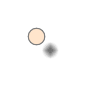
\begin{tikzpicture}
    \addtolength{\boxw}{\boxroundness * 2}
    \addtolength{\boxh}{\boxroundness * 2}

    \foreach \x in {0,.05,...,1}
    {
        \setlength{\tmpa}{\shadowsize * \real{\x}}
        \fill[xshift=\shadowsize - 1pt,yshift=-\shadowsize + 1pt,
                black,opacity=.04,rounded corners=\boxroundness]
            (\tmpa, \tmpa) rectangle +(\boxw - \tmpa - \tmpa,
                \boxh - \tmpa - \tmpa);
    }

    \filldraw[fill=lightorange, draw=black!50, rounded corners=\boxroundness]
        (0, 0) rectangle (\boxw, \boxh);
    \draw node[xshift=\boxroundness,yshift=\boxroundness,
        inner sep=1pt,outer sep=1pt,anchor=south west]
             (0,0) {\usebox{\shadowblockbox}};
\end{tikzpicture}}


%%%%%%%%5

\newcommand{\ceil}[1]{\left\lceil{#1}\right\rceil}

\newcommand{\optimize}[4]{%
  \begin{align}
    \min_{\substack{#2}}\quad & \label{opt:#1} #3 \\
    \text{subj. to}\quad & \nonumber #4
  \end{align}}

\newcommand{\optimizeoneline}[4]{%
  \begin{align}
    \min_{\substack{#2}}\quad & \label{opt:#1} #3 \quad
    \text{subj. to}\quad #4
  \end{align}}

\newcommand{\optimizemax}[4]{%
  \begin{align}
    \max_{\substack{#2}}\quad & \label{opt:#1} #3 \\
    \text{subj. to}\quad & \nonumber #4
  \end{align}}

\newcommand{\optimizemaxoneline}[4]{%
  \begin{align}
    \max_{\substack{#2}}\quad & \label{opt:#1} #3 \quad
    \text{subj. to}\quad #4
  \end{align}}

\newcommand{\optimizeuc}[3]{%
  \begin{align}
    \min_{\substack{#2}}\quad & \label{opt:#1} #3
  \end{align}}

\newcommand{\optimizeLagrange}[4]{%
  \begin{align}
    \max_{\substack{#2}} \min_{\substack{#3}}\quad & \label{opt:#1} #4
  \end{align}}

\newcommand{\optimizemaxuc}[3]{%
  \begin{align}
    \max_{\substack{#2}}\quad & \label{opt:#1} #3
  \end{align}}

\newcommand{\optimizemaxLagrange}[4]{%
  \begin{align}
    \min_{\substack{#2}} \max_{\substack{#3}}\quad & \label{opt:#1} #4
  \end{align}}

%\newtheorem{theorem}{Theorem}
%\newtheorem{definition}{Definitions}

%%% Local Variables: 
%%% mode: latex
%%% TeX-master: "courseml"
%%% End: 


\usepackage{times}
\usepackage[T1]{fontenc}
% Or whatever. Note that the encoding and the font should match. If T1
% does not look nice, try deleting the line with the fontenc.
\newcommand{\myalert}[1]{{%\color{red}
 #1}}
\iffalse

\chapter{Kernel Methods} \label{sec:kernel}

\chapterquote{}{}

\begin{learningobjectives}
\item Explain how kernels generalize both feature combinations and
  basis functions.
\item Contrast dot products with kernel products.
\item Implement kernelized perceptron.
\item Derive a kernelized version of regularized least squares
  regression.
\item Implement a kernelized version of the perceptron.
\item Derive the dual formulation of the support vector machine.
\end{learningobjectives}

\dependencies{}

\fi
\title[Kernel Methods]
{Kernel Methods}


%\author[F. Riguzzi] % (optional, use only with lots of authors)
%{Fabrizio Riguzzi}
% - Give the names in the same order as the appear in the paper.
% - Use the \inst{?} command only if the authors have different
%   affiliation.

\institute[] % (optional, but mostly needed)
{
%ENDIF -- University of Ferrara,  Italy\\
% fabrizio.riguzzi@unife.it
}
% - Use the \inst command only if there are several affiliations.
% - Keep it simple, no one is interested in your street address.
\date{}

\begin{document}
\begin{frame}
\titlepage 
\vspace{-2cm}
\begin{center}
Chapter 9 of ``A Course in  Machine Learning'' by Hal Daum\'e III

\url{http://ciml.info}

Conversion to beamer by Fabrizio Riguzzi
\end{center}

\end{frame}
  \renewcommand{\concept}[1]{\myalert{#1}}
  \renewcommand{\koncept}[2]{\myalert{#1}}

\renewcommand{\Figure}[3]{%
    \begin{center}
    \includegraphics[width=#3\textwidth]{../book/figs/#1}
    \end{center}
  }
  
\begin{frame}
  \frametitle{Kernel Methods}
\begin{itemize}
\item Linear models are great because they are easy to
understand and easy to optimize.
\item  They suffer because they can only
learn very simple decision boundaries.
\item  Neural networks can learn more
complex decision boundaries, but lose the nice convexity properties of
many linear models.
\end{itemize}
\end{frame}
\begin{frame}
  \frametitle{Kernel Methods}
\begin{itemize}
\item 
One way of getting a linear model to behave non-linearly is to
transform the input. 
\item For instance, by adding feature pairs as
additional inputs. 
\item Learning a linear model on such a representation
is convex, but is computationally prohibitive in all but very low
dimensional spaces. 
\item Instead of \emph{explicitly}
expanding the feature space, is it possible to stay with our original
data representation and do all the feature blow up \emph{implicitly?}
\item 
Surprisingly, the answer is often ``yes'' and the family of techniques
that makes this possible are known as \concept{kernel} approaches.
\end{itemize}
\end{frame}

\begin{comment}
   - From feature combinations and basis functions to kernels
   - Dot products versus kernels
   - Kernel/dual perceptron
   - Support vector machines
\end{comment}

%\section{From Feature Combinations to Kernels}

\begin{frame}
  \frametitle{From Feature Combinations to Kernels}
\begin{itemize}
\item 
Increasing the expressive power of linear models: explode the feature
space. 
\item For instance, a ``quadratic'' feature explosion might map a
feature vector $\vx = \langle x_1, x_2, x_3, \dots, x_D \rangle$ to an
expanded version denoted $\phi(\vx)$:
%
\begin{scriptsize}
\begin{align}
  \phi(\vx) = \langle &1, \sqrt 2x_1,\sqrt 2x_2,\sqrt 2x_3, \dots,\sqrt 2x_D, \nonumber\\
  & x_1^2, x_1 x_2, x_1 x_3, \dots, x_1 x_D, \nonumber\\
  & x_2 x_1, x_2^2, x_2 x_3, \dots, x_2 x_D, \nonumber\\
  & x_3 x_1, x_3 x_2, x_3^2, \dots, x_2 x_D, \nonumber\\
  & \dots, \nonumber\\
  & x_D x_1, x_D x_2, x_D x_3, \dots, x_D^2 \rangle
\end{align}
\end{scriptsize}
%
\item
(Note that there are repetitions here, but hopefully most learning
algorithms can deal well with redundant features; the reason for
$\sqrt 2x_i$ terms will be clear later.)
\end{itemize}
\end{frame}
\begin{frame}
  \frametitle{From Feature Combinations to Kernels}
\begin{itemize}
\item 
You could then train a classifier on this expanded feature space.
\item
There are two primary concerns in doing so.  The first is
computational: if your learning algorithm scales linearly in the
number of features, then you've just squared the amount of computation
you need to perform; you've also squared the amount of memory you'll
need.  
\item The second is statistical: if you go by the heuristic that you
should have about two examples for every feature, then you will now
need quadratically many training examples in order to avoid
overfitting.
\end{itemize}
\end{frame}
\begin{frame}
  \frametitle{From Feature Combinations to Kernels}
\begin{itemize}
\item We deal here  with the \emph{computational} issue.
\item You can also deal with
the statistical issue: for now, you can just hope that regularization
will be sufficient to attenuate overfitting.
\item
The key insight in kernel-based learning is that you can
\emph{rewrite} many linear models in a way that doesn't require you to
ever \emph{explicitly} compute $\phi(\vx)$. 
\end{itemize}
\end{frame}
\begin{frame}
  \frametitle{From Feature Combinations to Kernels}
\begin{itemize}
\item 
You can
think of this purely as a computational ``trick'' that enables you to
use the power of a quadratic feature mapping without actually having
to compute and store the mapped vectors.  
\item  Most algorithms we discuss involve
a product of the form $\dotp{\vw}{\phi(\vx)}$, after performing the
feature mapping.
\item  The goal is to rewrite these algorithms so that they
only ever depend on dot products between two examples, say $\vx$ and
$\vz$; namely, they depend on $\dotp{\phi(\vx)}{\phi(\vz)}$.
\end{itemize}
\end{frame}
\begin{frame}
  \frametitle{From Feature Combinations to Kernels}
\begin{itemize}
\item 
  To
understand why this is helpful, consider the quadratic expansion from
above, and the dot-product between two vectors.  You get:
%
\begin{scriptsize}
\begin{align}
\dotp{\phi(\vx)}{\phi(\vz)}
&= 1 + 2x_1 z_1 + 2x_2 z_2 + \dots + 2x_D z_D + x_1^2 z_1^2 + \dots + x_1 x_D z_1 z_D + \nonumber\\
&\quad \dots + x_D x_1 z_D z_1 + x_D x_2 z_D z_2 + \dots + x_D^2 z_D^2 \\
&= 1 + 2 \sum_d x_d z_d + \sum_d \sum_e x_d x_e z_d z_e \\
&= 1 + 2 \dotp{\vx}{\vz} + \left(\dotp{\vx}{\vz}\right)^2\\
&= (1 + \dotp{\vx}{\vz})^2
\end{align}
\end{scriptsize}
%
\item Thus, you can compute $\dotp{\phi(\vx)}{\phi(\vz)}$ in exactly the
same amount of time as you can compute $\dotp{\vx}{\vz}$ (plus the
time it takes to perform an addition and a multiply, about $0.02$
nanoseconds on a circa 2011 processor).
\end{itemize}
\end{frame}
\begin{frame}
  \frametitle{From Feature Combinations to Kernels}
\begin{itemize}
\item 
The rest of the practical challenge is to rewrite your algorithms so
that they only depend on dot products between examples and not on any
explicit weight vectors.
\end{itemize}
\end{frame}
%\section{Kernelized Perceptron}
\begin{frame}
  \frametitle{Kernelized Perceptron}
\newalgorithm%
  {kernel:perc}%
  {\FUN{PerceptronTrain}(\VAR{$\mat D$}, \VAR{MaxIter})}
  {
\SETST{$\vw$}{\CON{$\vec 0$}, \VAR{$b$} $\leftarrow$ \CON{0}}
  \COMMENT{initialize weights and bias}
\FOR{\VAR{iter} = \CON{1} \dots \VAR{MaxIter}}
\FORALL{(\VAR{$\vx$},\VAR{$y$}) $\in$ \VAR{$\mat D$}}
\SETST{$a$}{$\dotp{\VARm{\vw}}{\VARm{\phi(\vx)}} + \VARm{b}$}
  \COMMENT{compute activation for this example}
\IF{\VAR{$y$}\VAR{$a$} $\leq \CON{0}$}
\SETST{$\vw$}{\VAR{$\vw$} + \VAR{$y$} \VAR{$\phi(\vx)$}}
  \COMMENT{update weights}
\SETST{$b$}{\VAR{$b$} + \VAR{$y$}}
  \COMMENT{update bias}
\ENDIF
\ENDFOR
\ENDFOR
\RETURN \VAR{$\vw$}, \VAR{$b$}
}
\end{frame}
\begin{frame}
  \frametitle{Kernelized Perceptron}
\begin{itemize}
\item 
Consider the original perceptron algorithm 
 repeated above
using linear algebra notation and using feature expansion notation
$\phi(\vx)$. 
\item There are two places where
$\phi(\vx)$ is used explicitly.  The first is in computing the
activation (line 4) and the second is in updating the weights (line
6).  
\item The goal is to remove the explicit dependence of this algorithm
on $\phi$ and on the weight vector.
\end{itemize}
\end{frame}
\begin{frame}
  \frametitle{Kernelized Perceptron}
\begin{itemize}
\item 
  Reminder: if $\cU = \{ \vec u_i \}_l$ is a set of vectors in $\R^D$, then
  the span of $\cU$ is the set of vectors that can be written as
  linear combinations of $\vec u_i$s; namely: $\textit{span}(\cU) = \{
  \sum_i a_i \vec u_i : a_1 \in \R, \dots, a_I \in \R \}$.
\item 
  The null space of $\cU$ is everything that's left: $\R^D \without
  \textit{span}(\cU)$.
\end{itemize}
\end{frame}
\begin{frame}
  \frametitle{Kernelized Perceptron}
\begin{itemize}
\item 
You can observe that at any point in the algorithm, the
weight vector $\vw$ can be written as a linear combination of expanded
training data.
\item At any point, $\vw = \sum_n \al_n
\phi(\vx_n)$ for some parameters $\al$. 
\item Initially, $\vw = \vec 0$ so
choosing $\vec\al = 0$ yields this.  
\item If the first update occurs on the
$n$th training example, then the resolution weight vector is simply
$y_n \phi(\vx_n)$, which is equivalent to setting $\al_n = y_n$.
\item  If
the second update occurs on the $m$th training example, then all you
need to do is update $\al_m \leftarrow \al_m + y_m$.  
\end{itemize}
\end{frame}
\begin{frame}
  \frametitle{Kernelized Perceptron}
\begin{itemize}
\item 
This is true,
even if you make multiple passes over the data.  
\item This observation
leads to the following \concept{representer theorem}, which states
that the weight vector of the perceptron lies in the \concept{span} of
the training data.
\begin{theorem}[Perceptron Representer Theorem] \label{thm:kernel:perceptron}
  During a run of the perceptron algorithm, the weight vector $\vw$ is
  always in the span of the (assumed non-empty) training data,
  $\phi(\vx_1), \dots, \phi(\vx_N)$.
\end{theorem}
\end{itemize}
\end{frame}
\begin{frame}
  \frametitle{Kernelized Perceptron}
\begin{myproof}{\ref{thm:kernel:perceptron}}
  By induction.  Base case: the span of any non-empty set contains the
  zero vector, which is the initial weight vector.  Inductive case:
  suppose that the theorem is true before the $k$th update, and
  suppose that the $k$th update happens on example $n$.  By the
  inductive hypothesis, you can write $\vw = \sum_i \al_i \phi(\vx_i)$
  before the update.  The new weight vector is $\left[ \sum_i \al_i
    \phi(\vx_i) \right] + y_n \phi(\vx_n) = \sum_i (\al_i + y_n[i=n])
  \phi(\vx_i)$, which is still in the span of the training data.
\end{myproof}
\end{frame}
\begin{frame}
  \frametitle{Kernelized Perceptron}
\begin{itemize}
\item 
Now that you know that you can always write $\vw = \sum_n \al_n
\phi(\vx_n)$ for some $\al_i$s, you can additionally compute the
activations (line 4) as:
%
\begin{align}
\dotp{\vw}{\phi(\vx)}+b
&= \dotp{\left( \sum_n \al_n \phi(\vx_n) \right)}{\phi(\vx)} + b
\becauseof{definition of $\vw$} \\
&= \sum_n \al_n \Big[ \dotp{\phi(\vx_n)}{\phi(\vx)} \Big] + b
\becauseof{dot products are linear}
\end{align}
%
\item This now depends only on dot-products between data points, and never
explicitly requires a weight vector.
\item  You can now rewrite the entire
perceptron algorithm so that it never refers explicitly to the weights
and only ever depends on pairwise dot products between examples.
\end{itemize}
\end{frame}
\begin{frame}
  \frametitle{Kernelized Perceptron}
\newalgorithm%
  {kernel:kperc}%
  {\FUN{KernelizedPerceptronTrain}(\VAR{$\mat D$}, \VAR{MaxIter})}
  {
\SETST{$\vec\al$}{\CON{$\vec 0$}, \VAR{$b$} $\leftarrow$ \CON{0}}
  \COMMENT{initialize coefficients and bias}
\FOR{\VAR{iter} = \CON{1} \dots \VAR{MaxIter}}
\FORALL{(\VAR{$\vx_n$},\VAR{$y_n$}) $\in$ \VAR{$\mat D$}}
\SETST{$a$}{$\sum_m \al_m \dotp{\VARm{\phi(\vx_m)}}{\VARm{\phi(\vx_n)}} + \VARm{b}$}
  \COMMENT{compute activation for this example}
\IF{\VAR{$y_n$}\VAR{$a$} $\leq \CON{0}$}
\SETST{$\al_n$}{\VAR{$\al_n$} + \VAR{$y_n$}}
  \COMMENT{update coefficients}
\SETST{$b$}{\VAR{$b$} + \VAR{$y$}}
  \COMMENT{update bias}
\ENDIF
\ENDFOR
\ENDFOR
\RETURN \VAR{$\vec\al$}, \VAR{$b$}
}
\end{frame}
\begin{frame}
  \frametitle{Kernelized Perceptron}
\begin{itemize}
\item 
The advantage to this ``kernelized'' algorithm is that you can perform
feature expansions like the quadratic feature expansion from the
introduction for ``free.''
\item  For example, for exactly the same cost as
the quadratic features, you can use a \concept{cubic feature map},
computed as $\dotp{\phi(\vx)}{\phi(\vz)} = (1 + \dotp{\vx}{\vz})^3$,
which corresponds to three-way interactions between variables. 
\item In general, you can do so for any polynomial degree $p$ at the same
computational complexity.
\end{itemize}
\end{frame}
%\section{Kernelized K-means}
\begin{frame}
  \frametitle{Kernelized K-means}
\begin{itemize}
\item 
For a complete change of pace, consider the $K$-means algorithm
\item This algorithm is for \emph{clustering}
where there is no notion of ``training labels.''  
\item You want to
partition the data into coherent clusters. 
\item  For data in $\R^D$, it
involves randomly initializing $K$-many cluster means $\vec\mu\oth,
\dots, \vec\mu\Kth$.  
\item The algorithm then alternates between the
following two steps until convergence, with $\vx$ replaced by
$\phi(\vx)$ since that is the eventual goal:
\begin{enumerate}
\item For each example $n$, set cluster label $z_n = \arg\min_k
  \norm{\phi(\vx_n) - \vec\mu\kth}^2$.
\item For each cluster $k$, update $\vec\mu\kth = \frac 1 {N_k}
  \sum_{n : z_n=k} \phi(\vx_n)$, where $N_k$ is the number of $n$ with
  $z_n=k$.
\end{enumerate}
\end{itemize}
\end{frame}
\begin{frame}
  \frametitle{Kernelized K-means}
\begin{itemize}
\item 
The question is whether you can perform these steps without explicitly
computing $\phi(\vx_n)$. 
\item The \concept{representer theorem} is more
straightforward here than in the perceptron.
\item  The mean of a set of
data is, almost by definition, in the span of that data (choose the
$a_i$s all to be equal to $1/N$).  
\item Thus, so long as you
\emph{initialize} the means in the span of the data, you are
guaranteed always to have the means in the span of the data. 
\item  Given
this, you know that you can write each mean as an expansion of the
data; say that $\vec\mu\kth = \sum_n \al\kth_n \phi(\vx_n)$ for some
parameters $\al\kth_n$ (there are $N\times K$-many such parameters).
\end{itemize}
\end{frame}
\begin{frame}
  \frametitle{Kernelized K-means}
\begin{itemize}
\item 
Given this expansion, in order to execute step (1), you need to
compute norms.  This can be done as follows:
%
\begin{tiny}
\begin{align}
z_n 
&= \arg\min_k \norm{\textcolor{darkblue}{\phi(\vx_n)} - \textcolor{darkred}{\vec\mu\kth}}^2
   \becauseof{definition of $z_n$} \\
&= \arg\min_k \norm{\textcolor{darkblue}{\phi(\vx_n)} - \textcolor{darkred}{\sum_m \al\kth_m \phi(\vx_m)}}^2
   \becauseof{definition of $\vec\mu\kth$} \\
&= \arg\min_k \norm{\textcolor{darkblue}{\phi(\vx_n)}}^2+ \norm{\textcolor{darkred}{\sum_m \al\kth_m \phi(\vx_m)}}^2
   -2 \dotp{\textcolor{darkblue}{\phi(\vx_n)}}{\left[ \textcolor{darkred}{\sum_m \al\kth_m \phi(\vx_m)} \right]}
   \becauseof{expand quadratic term} \\
&= \arg\min_k \textcolor{darkred}{\sum_m \sum_{m'} \al\kth_m \al\kth_{m'} \dotp{\phi(\vx_m)}{\phi(\vx_{m'})}}
   -2 \textcolor{darkred}{\sum_m \al\kth_m} \dotp{\textcolor{darkred}{\phi(\vx_m)}}{\textcolor{darkblue}{\phi(\vx_n)}}
   + \textit{const}
   \becauseof{linearity and constant}
\end{align}
\end{tiny}
%
This computation can replace the assignments in step (1) of
$K$-means. 
\end{itemize}
\end{frame}
\begin{frame}
  \frametitle{Kernelized K-means}
\begin{itemize}
\item 
 The mean updates are more direct in step (2):
%
\begin{align}
\vec\mu\kth = \frac 1 {N_k} \sum_{n : z_n=k} \phi(\vx_n)
\quad\Longleftrightarrow\quad
\al\kth_n = \brack{\frac 1 {N_k} & \text{if } z_n = k \\ 0 & \text{otherwise}}
\end{align}
\end{itemize}
\end{frame}

%\section{What Makes a Kernel}
\begin{frame}
  \frametitle{What Makes a Kernel}
\begin{itemize}
\item 
A \concept{kernel} is just a form of generalized dot product.
\item  You can
also think of it as simply shorthand for
$\dotp{\phi(\vx)}{\phi(\vz)}$, which is commonly written
$K^\phi(\vx,\vz)$.
\item  Or, when $\phi$ is clear from context, simply
$K(\vx,\vz)$.
\item   This is often referred to as the kernel product between
$\vx$ and $\vz$ (under the mapping $\phi$).
\end{itemize}
\end{frame}

\begin{frame}
  \frametitle{What Makes a Kernel}
\begin{itemize}
\item 
In this view, what you've seen  is that
you can rewrite both the perceptron algorithm and the $K$-means
algorithm so that \emph{they only ever depend on kernel products
  between data points, and never on the actual datapoints themselves}.
\item
This is a very powerful notion, as it has enabled the development of a
large number of non-linear algorithms essentially ``for free'' (by
applying the so-called \concept{kernel trick}, that you've just seen
twice).
\end{itemize}
\end{frame}

\begin{frame}
  \frametitle{What Makes a Kernel}
\begin{itemize}
\item 
  If you have rewritten these
algorithms so that they only depend on the data through a function $K
: \cX \times \cX \fto \R$, can you stick \emph{any} function $K$ in
these algorithms, or are there some $K$ that are ``forbidden?'' 
\item In
one sense, you ``could'' use any $K$, but the real question is: for
what types of functions $K$ do these algorithms retain the properties
that we expect them to have (like convergence, optimality, etc.)?
\end{itemize}
\end{frame}

\begin{frame}
  \frametitle{What Makes a Kernel}
\begin{itemize}
\item 
One way to answer this question is to say that $K(\cdot,\cdot)$ is a
valid kernel if it corresponds to the inner product between two
vectors.
\item  That is, $K$ is valid if there exists a function $\phi$ such
that $K(\vx,\vz) = \dotp{\phi(\vx)}{\phi(\vz)}$. 
\item This is a direct
definition and it should be clear that if $K$ satisfies this, then the
algorithms go through as expected (because this is how we derived
them).
\end{itemize}
\end{frame}

\begin{frame}
  \frametitle{What Makes a Kernel}
\begin{itemize}
\item 
You've already seen the general class of \concept{polynomial kernels},
which have the form:
%
\begin{align}
K\xth{poly}_d(\vx,\vz) &= \Big( 1 + \dotp{\vx}{\vz} \Big)^d
\end{align}
%
where $d$ is a hyperparameter of the kernel.  
\item These kernels correspond
to polynomial feature expansions.
\end{itemize}
\end{frame}

\begin{frame}
  \frametitle{What Makes a Kernel}
\begin{itemize}
\item 
There is an alternative characterization of a valid kernel function
that is more mathematical.
\item  It states that $K : \cX \times \cX \fto
\R$ is a kernel if $K$ is \concept{positive semi-definite} (or, in
shorthand, \concept{psd}). 
\item This property is also sometimes called
\concept{Mercer's condition}.  
\item This means the
\emph{for all} functions $f$ that are square integrable (i.e., $\int
f(\vx)^2 \ud\vx < \infty$), other than the zero function, the
following property holds:
%
\begin{align}
\int\!\!\!\int f(\vx) K(\vx,\vz) f(\vz) \ud \vx \ud \vz > 0
\end{align}
%
\end{itemize}
\end{frame}

\begin{frame}
  \frametitle{What Makes a Kernel}
\begin{itemize}
\item 
This likely seems like it came out of nowhere. 
\item The
connection is well beyond the scope of this treatment, but is covered well
is external sources.
\item  For now, simply take it as a given that this is
an equivalent requirement.
%\end{itemize}
%\end{frame}
%
%\begin{frame}
%  \frametitle{What Makes a Kernel}
%\begin{itemize}
\item 
The question is: why is this alternative characterization useful? 
\item It
is useful because it gives you an alternative way to construct kernel
functions.
\end{itemize}
\end{frame}

\begin{frame}
  \frametitle{What Makes a Kernel}
\begin{itemize}
\item Using it you can easily prove the following,
which would be difficult from the definition of kernels as inner
products after feature mappings.
%
\begin{theorem}[Kernel Addition] \label{thm:kernel:addition}
  If $K_1$ and $K_2$ are kernels, the $K$ defined by $K(\vx,\vz) =
  K_1(\vx,\vz) + K_2(\vx,\vz)$ is also a kernel.
\end{theorem}
\end{itemize}
\end{frame}

\begin{frame}
  \frametitle{What Makes a Kernel}
\begin{myproof}{\ref{thm:kernel:addition}}
You need to verify the positive semi-definite property on $K$.  You
can do this as follows:
%
\begin{footnotesize}
\begin{align}
\int\!\!\!\int f(\vx) K(\vx,\vz) f(\vz) \ud \vx \ud \vz \\
= \int\!\!\!\int f(\vx) \left[ K_1(\vx,\vz) + K_2(\vx,\vz) \right] f(\vz) \ud \vx \ud \vz 
   \becauseof{definition of $K$}\\
= \int\!\!\!\int f(\vx) K_1(\vx,\vz) f(\vz) \ud \vx \ud \vz \nonumber\\
\quad + \int\!\!\!\int f(\vx) K_2(\vx,\vz) f(\vz) \ud \vx \ud \vz 
  \becauseof{distributive rule}\\
> 0 + 0
   \becauseof{$K_1$ and $K_2$ are psd}
\end{align}
\end{footnotesize}
\end{myproof}
\end{frame}

\begin{frame}
  \frametitle{What Makes a Kernel}
\begin{itemize}
\item 
More generally, any positive linear combination of kernels is still a
kernel.
\item  Specifically, if $K_1, \dots, K_M$ are all kernels, and
$\al_1, \dots, \al_M \geq 0$, then $K(\vx,\vz) = \sum_m \al_m
K_m(\vx,\vz)$ is also a kernel.
\item 
You can also use this property to show that the following
\concept{Gaussian kernel} (also called the \concept{RBF kernel}) is
also psd:
%
\begin{align}
K\xth{RBF}_\ga(\vx,\vz) &= \exp\left[ - \ga \norm{\vx-\vz}^2 \right]
\end{align}
%
\item
Here $\ga$ is a hyperparameter that controls the width of this
Gaussian-like bumps. 
\end{itemize}
\end{frame}

\begin{frame}
  \frametitle{What Makes a Kernel}
\begin{itemize}
\item 
 To gain an intuition for what the RBF kernel is
doing, consider what prediction looks like in the perceptron:
%
\begin{align}
f(\vx) &= \sum_n \al_n K(\vx_n, \vx) + b \\
&= \sum_n \al_n \exp\left[ - \ga \norm{\vx_n-\vz}^2 \right]
\end{align}
%
\item In this computation, each training example is getting to ``vote'' on
the label of the test point $\vx$.
\item  The amount of ``vote'' that the
$n$th training example gets is proportional to the negative
exponential of the distance between the test point and itself. 
\item This
is very much like an RBF neural network, in which there is a Gaussian
``bump'' at each training example
%, with variance $1/(2\ga)$, and 
where
the $\al_n$s act as the weights connecting these RBF bumps to the
output.
\end{itemize}
\end{frame}

\begin{frame}
  \frametitle{What Makes a Kernel}
\begin{itemize}
\item 
Showing that this kernel is positive definite is a bit of an exercise
in analysis (particularly, integration by parts), but otherwise not
difficult.
\end{itemize}
\end{frame}

\begin{frame}
  \frametitle{What Makes a Kernel}
\begin{itemize}
\item 
You have seen two basic classes of kernels: polynomial kernels
($K(\vx,vz) = (1 + \dotp{\vx}{\vz})^d$), which includes the linear
kernel ($K(\vx,\vz) = \dotp{\vx}{\vz}$) and RBF kernels ($K(\vx,\vz) =
\exp[-\ga \norm{\vx-\vz}^2]$). 
\item  The former have a direct connection to
feature expansion; the latter to RBF networks.  
\item You also know how to
combine kernels to get new kernels by addition.  
\item You can do
more than that: the product of two kernels is also a kernel.
\end{itemize}
\end{frame}

\begin{frame}
  \frametitle{What Makes a Kernel}
\begin{itemize}
\item 
As far as a ``library of kernels'' goes, there are many.  
\item Polynomial
and RBF are by far the most popular. 
\item A commonly used, but technically
\emph{invalid} kernel, is the hyperbolic-tangent kernel, which mimics
the behavior of a two-layer neural network.  It is defined as:
%
\begin{align}
K\xth{tanh} &= \tanh(1 + \dotp{\vx}{\vz})
\becauseof{Warning: not psd}
\end{align}
\end{itemize}
\end{frame}

\begin{frame}
  \frametitle{What Makes a Kernel}
\begin{itemize}
\item 
A final example, which is not very common, but is nonetheless
interesting, is the all-subsets kernel. 
\item Suppose that your $D$
features are all \emph{binary}: all take values $0$ or $1$.  
\item Let $A
\subseteq \{ 1, 2, \dots D \}$ be a subset of features, and let
$f_A(\vx) = \bigwedge_{d \in A} x_d$ be the conjunction of all the
features in $A$.  
\item Let $\phi(\vx)$ be a feature vector over \emph{all}
such $A$s, so that there are $2^D$ features in the vector $\phi$.  
\end{itemize}
\end{frame}

\begin{frame}
  \frametitle{What Makes a Kernel}
\begin{itemize}
\item 
You
can compute the kernel associated with this feature mapping as:
%
\begin{align}
K\xth{subs}(\vx,\vz) &= \prod_d \Big( 1 + x_d z_d \Big)
\end{align}
%
\item Verifying the relationship between this kernel and the all-subsets
feature mapping is left as an exercise (but closely resembles the
expansion for the quadratic kernel).
\end{itemize}
\end{frame}
%\section{Support Vector Machines}

\begin{frame}
  \frametitle{Support Vector Machines}
\begin{itemize}
\item 
Kernelization predated support vector machines, but SVMs are
definitely the model that popularized the idea.
\item   Recall the definition
of the soft-margin SVM and in
particular the optimization problem which
attempts to balance a \textcolor{darkblue}{large margin} (small
$\norm{\vw}^2$) with a \textcolor{darkergreen}{small loss} (small
$\xi_n$s, where $\xi_n$ is the \concept{slack} on the $n$th training
example).  
\item This problem is repeated below:
%
\optimize{kernel:svm}{\vw,b,\vec\xi}{%
  \textcolor{darkblue}{\frac 1 2 \norm{\vw}^2}
+ \textcolor{darkergreen}{C \sum_n \xi_n}
}{%
  \textcolor{darkred}{y_n \left( \dotp{\vw}{\vx_n} + b \right) \geq 1 - \xi_n} & (\forall n) \\
\nonumber &
  \textcolor{darkpurple}{\xi_n \geq 0} & (\forall n)
}
\end{itemize}
\end{frame}

\begin{frame}
  \frametitle{Support Vector Machines}
\begin{itemize}
\item 
%
Previously, you optimized this by explicitly computing the slack
variables $\xi_n$, given a solution to the decision boundary, $\vw$
and $b$.
\item  You can use Lagrange
multipliers to optimize constrained problems. 
\item The overall \emph{goal}
is going to be to rewrite the SVM optimization problem in a way that
it no longer explicitly depends on the weights $\vw$ and only depends
on the examples $\vx_n$ through kernel products.
\end{itemize}
\end{frame}

\begin{frame}
  \frametitle{Support Vector Machines}
\begin{itemize}
\item 
There are $2N$ constraints in this optimization, one for each slack
constraint and one for the requirement that the slacks are
non-negative.
%\item  Unlike the last time, these constraints are now
%\emph{inequalities}, which require a slightly different solution.
\item
First, you rewrite all the inequalities so that they read as
$\textit{something} \geq 0$ and then add corresponding Lagrange
multipliers.
\item   Lagrange multipliers are
constrained to be non-negative, and their sign in the augmented
objective function matters.
\end{itemize}
\end{frame}

\begin{frame}
  \frametitle{Support Vector Machines}
\begin{itemize}
\item 
The second set of constraints is already in the proper form.
\item The first
set can be rewritten as $\textcolor{darkred}{y_n \left(
    \dotp{\vw}{\vx_n} + b \right) - 1 + \xi_n \geq 0}$.  
    \item You're now
ready to construct the Lagrangian, using multipliers $\al_n$ for the
first set of constraints and $\be_n$ for the second set.
%
\begin{align}
\cL(\vw,b,\vec\xi,\vec\al,\vec\be)
&= 
  \textcolor{darkblue}{\frac 1 2 \norm{\vw}^2}
%\\&\qquad
+ \textcolor{darkergreen}{C \sum_n \xi_n}
%\\&\qquad
- \sum_n \be_n \textcolor{darkpurple}{\xi_n}
\\&\qquad
- \sum_n \al_n \left[
    \textcolor{darkred}{y_n \left( \dotp{\vw}{\vx_n} + b \right) - 1 + \xi_n}
  \right] 
\end{align}
%
\end{itemize}
\end{frame}

\begin{frame}
  \frametitle{Support Vector Machines}
\begin{itemize}
\item 
The \emph{new} optimization problem is:
%
\begin{align}
\min_{\vw,b,\vec\xi} \max_{\vec\al \geq 0} \max_{\vec\be \geq 0} \cL(\vw,b,\vec\xi,\vec\al,\vec\be)
\end{align}
%
\end{itemize}
\end{frame}

\begin{frame}
  \frametitle{Support Vector Machines}
\begin{itemize}
\item 
The intuition is exactly the same as before. 
\item If you are able to find
a solution that satisfies the constraints (e.g., the purple term is
properly non-negative), then the $\be_n$s cannot do anything to
``hurt'' the solution. 
\item On the other hand, if the purple term
\emph{is} negative, then the corresponding $\be_n$ can go to
$+\infty$, breaking the solution.
\end{itemize}
\end{frame}

\begin{frame}
  \frametitle{Support Vector Machines}
\begin{itemize}
\item 
You can solve this problem by taking gradients.  
\item  Since your goal is to remove the dependence on $\vw$, the
first step is to take a gradient with respect to $\vw$, set it equal
to zero, and solve for $\vw$ in terms of the other variables.
%
\begin{align}
\grad_{\vw} \cL
= \textcolor{darkblue}{\vw} 
  - \sum_n \al_n \textcolor{darkred}{y_n \vx_n}
= 0 \quad\Longleftrightarrow\quad
\textcolor{darkblue}{\vw} 
= \sum_n \al_n \textcolor{darkred}{y_n \vx_n}
\end{align}
%
\item
At this point, you should immediately recognize a similarity to the
kernelized perceptron: the optimal weight vector takes \emph{exactly}
the same form in both algorithms.
\end{itemize}
\end{frame}

\begin{frame}
  \frametitle{Support Vector Machines}
\begin{itemize}
\item 
You can now take this new expression for $\vw$ and plug it back in to
the expression for $\cL$, thus removing $\vw$ from consideration.  
\item To
avoid subscript overloading, you should replace the $n$ in the
expression for $\vw$ with, say, $m$.  This yields:
%
\begin{align}
\cL(b,\vec\xi,\vec\al,\vec\be)
&= 
  \textcolor{darkblue}{\frac 1 2 \norm{\sum_m \al_m y_m \vx_m}^2}
%\\&\qquad
+ \textcolor{darkergreen}{C \sum_n \xi_n}
%\\&\qquad
- \sum_n \be_n \textcolor{darkpurple}{\xi_n}
\\&\qquad
- \sum_n \al_n \left[
    \textcolor{darkred}{y_n \left( \dotp{\left[ \sum_m \al_m y_m \vx_m\right]}{\vx_n} + b \right) - 1 + \xi_n}
  \right]
\end{align}
%
\end{itemize}
\end{frame}

\begin{frame}
  \frametitle{Support Vector Machines}
\begin{itemize}
\item 
At this point, it's convenient to rewrite these terms; be sure you
understand where the following comes from:
%
\begin{small}
\begin{align}
\cL(b,\vec\xi,\vec\al,\vec\be)
&= 
  \textcolor{darkblue}{\frac 1 2
    \sum_n \sum_m \al_n \al_m y_n y_m \dotp{\vx_n}{\vx_m}
  }
+ \sum_n (\textcolor{darkergreen}{C} - \textcolor{darkpurple}{\be_n}) \xi_n
\\&\qquad
   - \textcolor{darkred}{
    \sum_n
    \sum_m 
      \al_n \al_m y_n y_m \dotp{\vx_n}{\vx_m}
}
- \textcolor{darkred}{
  \sum_n \al_n \left( y_n b - 1 + \xi_n \right)}\\
&=
-   \textcolor{darkblue}{\frac 1 2
    \sum_n \sum_m \al_n \al_m y_n y_m \dotp{\vx_n}{\vx_m}
  }
+ \sum_n (\textcolor{darkergreen}{C} - \textcolor{darkpurple}{\be_n}) \xi_n
\\&\qquad
\textcolor{darkred}{
-  b \sum_n \al_n y_n 
-  \sum_n \al_n (\xi_n - 1)}
\end{align}
\end{small}
%
\end{itemize}
\end{frame}

\begin{frame}
  \frametitle{Support Vector Machines}
\begin{itemize}
\item 
Things are starting to look good: you've successfully removed the
dependence on $\vw$, \emph{and} everything is now written in terms of
dot products between input vectors!  
\item This might still be a difficult
problem to solve, so you need to continue and attempt to remove the
remaining variables $b$ and $\vec \xi$.
\end{itemize}
\end{frame}

\begin{frame}
  \frametitle{Support Vector Machines}
\begin{itemize}
\item 
The derivative with respect to $b$ is:
%
\begin{align}
\partialof{\cL}{b}
&= - \sum_n \al_n y_n = 0
\end{align}
%
\item
This doesn't allow you to \emph{substitute} $b$ with something (as you
did with $\vw$), but it does mean that the fourth term ($b \sum_n
\al_n y_n$) goes to zero at the optimum.
\end{itemize}
\end{frame}

\begin{frame}
  \frametitle{Support Vector Machines}
\begin{itemize}
\item 
The last of the original variables is $\xi_n$; the derivatives in this
case look like:
%
\begin{align}
\partialof{\cL}{\xi_n}
&= C - \be_n - \al_n
\quad \Longleftrightarrow \quad
C - \be_n = \al_n
\end{align}
%
\item
Again, this doesn't allow you to substitute, but it does mean that you
can rewrite the second term, which is $\sum_n (C-\be_n)\xi_n$, as
$\sum_n \al_n \xi_n$. 
\item This then cancels with (most of) the final
term. 
\end{itemize}
\end{frame}

\begin{frame}
  \frametitle{Support Vector Machines}
\begin{itemize}
\item 
 However, you need to be careful to remember something.
 \item  When we
optimize, both $\al_n$ and $\be_n$ are constrained to be non-negative.
\item What this means is that since we are dropping $\be$ from the
optimization, we need to ensure that $\al_n \leq C$, otherwise the
corresponding $\be$ will need to be negative, which is not allowed.
\end{itemize}
\end{frame}

\begin{frame}
  \frametitle{Support Vector Machines}
\begin{itemize}
\item 
You finally wind up with the following, where $\dotp{\vx_n}{\vx_m}$
has been replaced by $K(\vx_n,\vx_m)$:
%
\begin{align}
\cL(\vec\al)
&=
\sum_n \al_n
- \frac 1 2
    \sum_n \sum_m \al_n \al_m y_n y_m K(\vx_n,\vx_m)
\end{align}
%
\item 
If you are comfortable with matrix notation, this has a very compact
form. 
\end{itemize}
\end{frame}

\begin{frame}
  \frametitle{Support Vector Machines}
\begin{itemize}
\item 
 Let $\vec 1$ denote the $N$-dimensional vector of all $1$s, 
let $\vec y$ denote the vector of labels and let $\mat G$ be the $N
\times N$ matrix, where $\mat G_{n,m} = y_n y_m K(\vx_n, \vx_m)$, then this
has the following form:
%
\begin{align}
\cL(\vec\al)
&=
\vec\al\T\vec 1
- \frac 1 2 \vec\al\T \mat G \vec\al
\end{align}
%
\end{itemize}
\end{frame}

\begin{frame}
  \frametitle{Support Vector Machines}
\begin{itemize}
\item 
The resulting optimization problem is to \emph{maximize}
$\cL(\vec\al)$ as a function of $\vec\al$, subject to the constraint
that the $\al_n$s are all non-negative and less than $C$ (because of
the constraint added when removing the $\be$ variables).  
\item Thus, your
problem is:
%
\optimize{kernel:svmdual}{\vec\al}{%
- \cL(\vec \al) = 
\frac 1 2
    \sum_n \sum_m \al_n \al_m y_n y_m K(\vx_n,\vx_m)
- \sum_n \al_n
}{%
  0 \leq \al_n \leq C & (\forall n)
}
%
\end{itemize}
\end{frame}

\begin{frame}
  \frametitle{Support Vector Machines}
\begin{itemize}
\item 
One way to solve this problem is gradient descent on $\al$.  
\item The only
complication is making sure that the $\al$s satisfy the constraints.
\item In this case, you can use a \concept{projected gradient} algorithm:
after each gradient update, you adjust your parameters to satisfy the
constraints by \emph{projecting} them into the feasible region. 
\item In
this case, the projection is trivial: if, after a gradient step, any
$\al_n < 0$, simply set it to $0$; if any $\al_n > C$, set it to $C$.
\end{itemize}
\end{frame}
%\section{Understanding Support Vector Machines}

\begin{frame}
  \frametitle{Understanding Support Vector Machines}
\begin{itemize}
\item 
The prior discussion involved quite a bit of math to derive a
representation of the support vector machine in terms of the Lagrange
variables.
\item  This mapping is actually sufficiently standard that
everything in it has a name. 
\item The original problem variables
($\vw,b,\vec\xi$) are called the \concept{primal variables}; 
\item The
Lagrange variables are called the \concept{dual variables}. 
\item The
optimization problem that results after removing all of the primal
variables is called the \concept{dual problem}.
\end{itemize}
\end{frame}

\begin{frame}
  \frametitle{Understanding Support Vector Machines}
\begin{itemize}
\item 
A succinct way of saying what you've done is: you found that after
converting the SVM into its dual, it is possible to kernelize.
\item
To understand SVMs, a first step is to peek into the dual formulation,
Eq~\eqref{opt:kernel:svmdual}.
\item  The objective has two terms: the first
depends on the data, and the second depends only on the dual
variables.
\item  The first thing to notice is that, because of the second
term, the $\al$s ``want'' to get as large as possible.  
\item The constraint
ensures that they cannot exceed $C$, which means that the general
tendency is for the $\al$s to grow as close to $C$ as possible.
\end{itemize}
\end{frame}

\begin{frame}
  \frametitle{Understanding Support Vector Machines}
\begin{itemize}
\item 
To further understand the dual optimization problem, it is useful to
think of the kernel as being a measure of \emph{similarity} between
two data points.
\item  This analogy is most clear in the case of RBF
kernels, but even in the case of linear kernels, if your examples all
have unit norm, then their dot product is still a measure of
similarity.
\item  Since you can write the prediction function as $f(\hat \vx)
= \sign( \sum_n \al_n y_n K(\vx_n,\hat \vx) )$, it is natural to think
of $\al_n$ as the ``importance'' of training example $n$, where $\al_n
= 0$ means that it is not used at all at test time.
\end{itemize}
\end{frame}

\begin{frame}
  \frametitle{Understanding Support Vector Machines}
\begin{itemize}
\item 
Consider two data points that have the same label; namely, $y_n =
y_m$.  
\item This means that $y_n y_m = +1$ and the objective function has a
term that looks like $\al_n \al_m K(\vx_n, \vx_m)$.  
\item Since the goal is to
make this term small, then one of two things has to happen: either $K$
has to be small, or $\al_n \al_m$ has to be small.
\item  If $K$ is already
small, then this doesn't affect the setting of the corresponding
$\al$s.
\end{itemize}
\end{frame}

\begin{frame}
  \frametitle{Understanding Support Vector Machines}
\begin{itemize}
\item  But if $K$ is large, then this \emph{strongly} encourages at
least one of $\al_n$ or $\al_m$ to go to zero.  
\item So if you have two
data points that are very similar \emph{and} have the same label, at
least one of the corresponding $\al$s will be small. 
\item This makes
intuitive sense: if you have two data points that are basically the
same (both in the $\vx$ and $y$ sense) then you only need to ``keep''
one of them around.
\end{itemize}
\end{frame}

\begin{frame}
  \frametitle{Understanding Support Vector Machines}
\begin{itemize}
\item 
Suppose that you have two data points with different labels: $y_n y_m
= -1$.
\item  Again, if $K(\vx_n,\vx_m)$ is small, nothing happens.  
\item But if
it is large, then the corresponding $\al$s are encouraged to be as
large as possible. 
\item In other words, if you have two similar examples
with different labels, you are strongly encouraged to keep the
corresponding $\al$s as large as $C$.
\end{itemize}
\end{frame}

\begin{frame}
  \frametitle{Understanding Support Vector Machines}
\begin{itemize}
\item 
An alternative way of understanding the SVM dual problem is
geometrically.
\item  Remember that the whole point of introducing the
variable $\al_n$ was to ensure that the $n$th training example was
correctly classified, modulo slack. 
\item More formally, the goal of
$\al_n$ is to ensure that $y_n (\dotp{\vw}{\vx_n}+b) - 1 + \xi_n \geq 0$.
\item Suppose that this constraint is \emph{not} satisfied. 
\item There is an
important result in optimization theory, called the
\concept{Karush-Kuhn-Tucker conditions} (or \concept{KKT conditions},
for short), that states that at the optimum, the product of the
Lagrange multiplier for a constraint, and the value of that
constraint, will equal zero. 
\end{itemize}
\end{frame}

\begin{frame}
  \frametitle{Understanding Support Vector Machines}
\begin{itemize}
\item 
 In this case, this says that at the
optimum, you have:
%
\begin{align}
  \al_n \Big[ y_n \left( \dotp{\vw}{\vx_n} + b \right) - 1 + \xi_n \Big] = 0
\end{align}
%
\item In order for this to be true, it means that (at least) one of the
following must be true:
%
\begin{align}
  \al_n = 0 \qquad{\textit{or}}\qquad
  y_n \left( \dotp{\vw}{\vx_n} + b \right) - 1 + \xi_n = 0
\end{align}
%
\end{itemize}
\end{frame}

\begin{frame}
  \frametitle{Understanding Support Vector Machines}
\begin{itemize}
\item 
A reasonable question to ask is: under what circumstances will $\al_n$
be \emph{non-zero?}  
\item From the KKT conditions, you can discern that
$\al_n$ can be non-zero \emph{only} when the constraint holds
\emph{exactly}; namely, that $y_n \left( \dotp{\vw}{\vx_n} + b \right)
- 1 + \xi_n = 0$.
\item  When does that constraint hold \emph{exactly}? 
\item It
holds exactly only for those points \emph{precisely} on the margin of
the hyperplane.
\end{itemize}
\end{frame}

\begin{frame}
  \frametitle{Understanding Support Vector Machines}
\begin{itemize}
\item 
In other words, the \emph{only} training examples for which $\al_n
\neq 0$ are those that lie precisely $1$ unit away from the maximum
margin decision boundary! 
\item (Or those that are ``moved'' there by the
corresponding slack.) 
\item These points are called the \concept{support
  vectors} because they ``support'' the decision boundary. 
  \item In
general, the number of support vectors is far smaller than the number
of training examples, and therefore you naturally end up with a
solution that only uses a subset of the training data.
\end{itemize}
\end{frame}

\begin{frame}
  \frametitle{Understanding Support Vector Machines}
\begin{itemize}
\item 
From the first discussion, you know that the points that wind up being
support vectors are exactly those that are ``confusable'' in the sense
that you have  examples that are nearby, but have different labels.
\item
This is a completely in line with the previous discussion.  
\item If you
have a decision boundary, it will pass between these ``confusable''
points, and therefore they will end up being part of the set of
support vectors.
\end{itemize}
\end{frame}

\end{document}
\begin{comment}
%\section{Kernelized Regression}

Now, consider another example: linear regression 
\item This was a linear model, under which $y
= \dotp{\vw}{\vx}+b$ and where the optimal weights are given in closed
form by:
%
\begin{align}
  \textcolor{darkred}{\vw} &= \textcolor{darkblue}{\left( \mat X \T \mat X + \la \eye_D \right)}\inv \textcolor{darkergreen}{\mat X \T \vec Y}
\end{align}
%
where $\mat X$ is the $N\times D$ data matrix, $\la$ is a
regularization parameter and $\vec Y$ is the $N\times 1$ vector of
labels.

This algorithm is, in some ways, even easier to kernelize than the
perceptron.  The optimal solution has a closed form, and 
\end{comment}

% http://www.ics.uci.edu/~welling/classnotes/papers_class/Kernel-Ridge.pdf
% http://crsouza.blogspot.com/2010/03/kernel-functions-for-machine-learning.html#exponential
% http://nlp.stanford.edu/IR-book/html/htmledition/nonlinear-svms-1.html

\begin{exercises}
\begin{Ex}
\TODO

\begin{solution}
\TODO
\end{solution}
\end{Ex}

\end{exercises}

%%% Local Variables: 
%%% mode: latex
%%% TeX-master: "courseml"
%%% End:
